% Load LaTeX and package
\documentclass[11pt, xcolor=x11names,compress]{beamer}
\usepackage[utf8]{inputenc}
\usepackage{mathtools}  % for paired delimiters 
\usepackage{mathrsfs}   % for script capitals
\usepackage{amsmath}
\usepackage{amssymb}
\usepackage{amsfonts}

\usepackage[dvipsnames]{xcolor} % for color
\usepackage{ragged2e} % for text alignment
\usepackage{dsfont} % for sepecial font (mathds)

\usepackage[labelformat=empty]{caption}

\usepackage{natbib}
\bibliographystyle{abbrvnat}
% Customize theme attributes
\setbeamertemplate{headline}[default]
%% Hide navigation symbols
\setbeamertemplate{navigation symbols}{}
%%\mode<beamer>{\setbeamertemplate{blocks}[rounded][shadow=true]} %for block
%% Outer theme
\useoutertheme{infolines}
\useoutertheme[subsection=false]{miniframes}

%% Inner theme
\useinnertheme{}

% Define template colors
\usecolortheme{rose}
%\usecolortheme{default}

\definecolor{UniColor}{RGB}{0,0, 255}
\setbeamercolor{structure}{bg=white, fg=UniColor}
\setbeamercolor{title}{bg = white, fg = UniColor}
\setbeamercolor{author}{bg = white, fg = UniColor}

\DeclareMathOperator{\Var}{\text{Var}}
\DeclareMathOperator{\E}{\text{E}}
\DeclareMathOperator{\Cov}{\text{Cov}}
\DeclareMathOperator{\Corr}{\text{Corr}}

%------------------------------------------------------------
%This block of code defines the information to appear in the
%Title page


\title [ECON 4003: Empirical Exercise 6]{ECON 4003 Econometrics I}

\vspace{10mm}

\author[]{Empirical Exercise 6}
\date[]{\textit{By Duong Trinh}}

%End of title page configuration block
%---------------------------------------------------- 

\begin{document}
\setbeamertemplate{caption}[numbered]
%The next statement creates the title page.
{\titlegraphic{
\includegraphics[scale = 0.05]{GlaLogo.pdf}}
\frame{\titlepage}}
\linespread{1.15}
%---------------------------------------------------------

\begin{frame}[fragile,t]
\linespread{1.3}
\frametitle{Picture the Scenario}
\begin{itemize}
    \item \textbf{Objective:} Investigate the impact of the \textbf{marginal tax rate} paid by high-income earners on the level of \textbf{inequality}.
    \item \textbf{Data:} Time-series data on five different countries
    \begin{itemize}
        \item[$\square$] We use a subset of their data for Australia can be found in the file \texttt{inequality\_aus.dta}.
    \end{itemize}
    \item \textbf{Key variables:}
    \begin{itemize}
        \item[$\square$] \texttt{share}: the percentage income share
of the top 1\% of incomes.
        \item[$\square$] \texttt{tax}: the median marginal tax rate (as a percentage) paid on wages by the top 1\% of income earners.
        \item[$\square$] \texttt{year}: $1 = 1921, 2 = 1922, ... , 80 = 2000$.
        \item[$\square$] \texttt{gwth}: the percentage growth rate
    \end{itemize}
\end{itemize}
\end{frame}
%---------------------------------------------------------

%---------------------------------------------------------
\begin{frame}
\frametitle{Question (a)}
\begin{itemize}
    \item Estimate the equation: $share = \beta_0 + \beta_1tax + u$
    \item Interpret your estimate for $\beta_1$.\\
    Would you interpret this as a causal relationship?\\
    Is the OLS estimator $\widehat{\beta}_1$ unbiased?\\
\pause
\vspace{10mm}
\textit{Answer.}\\
\begin{equation*}
    \underset{(se)}{\widehat{share}} = \underset{(0.2358)}{12.0207} - \underset{(0.005336)}{0.1044} \cdot tax
\end{equation*}
\begin{equation*}
    R^2=0.6668 \quad SER=1.346
\end{equation*}
\end{itemize}
\end{frame}
%---------------------------------------------------------

%---------------------------------------------------------
\begin{frame}[fragile,t]
\frametitle{Question (b)}
\begin{itemize}
    \item It is generally recognized that inequality was high prior to the great depression, then declined during the depression and World War II, increasing again toward the end of the sample period. To capture this effect, estimate the following model with a linear trend:
    $$share = \beta_0 + \beta_1tax + \beta_2year + \epsilon$$
\end{itemize}
\end{frame}
%---------------------------------------------------------

%---------------------------------------------------------
\begin{frame}[fragile,t]
\frametitle{Question (b)}
\begin{itemize}
    \item Interpret the estimates for $\beta_1$ and $\beta_2$. Are the estimates statistically significant?\\
\pause
\begin{equation*}
    \underset{(se)}{\widehat{share}} = \underset{(0.2261)}{12.0370} - \underset{(0.01627)}{0.07467} \cdot tax - \underset{(0.01456)}{0.02776}\cdot year \quad R^2=0.69 \quad SER = 1.31
\end{equation*}
\begin{itemize}
    \item [$\square$] Controlling for time trend, we find that an increase in the marginal tax rate for top earners by one percentage is associated with a decrease in the income share of the top earners by 0.07467 percentage on average. The p-value is 0.000; therefore, the estimate is statistically significant at 1\% significance level.
    \item [$\square$] Holding marginal tax rate constant, the income share of the top earners decreases by 0.02776 percentage per year on average. \\
    The p-value is 0.060; therefore, the estimate is statistically significant at 10\% significance level.
\end{itemize}
\end{itemize}
\end{frame}
%---------------------------------------------------------

%---------------------------------------------------------
\begin{frame}[fragile,t]
\frametitle{Question (b)(cont.)}
\begin{itemize}
    \item Has adding the trend changed estimated coefficient for \texttt{tax}?\\
\pause
\vspace{5mm}
\textit{Answer.}
\begin{equation*}
    \underset{(se)}{\widehat{share}} = \overset{\hat{\beta}_0}{\underset{(0.2358)}{12.0207}} - \overset{\hat{\beta}_1}{\underset{(0.005336)}{0.1044}} \cdot tax
\end{equation*}
\begin{equation*}
    R^2=0.6668 \quad SER=1.346
\end{equation*}
\vspace{2mm}
\begin{equation*}
    \underset{(se)}{\widehat{share}} = \overset{\hat{\beta}_0^*}{\underset{(0.2261)}{12.0370}} - \overset{\hat{\beta}_1^*}{\underset{(0.01627)}{0.07467}} \cdot tax - \overset{\hat{\beta}_2^*}{\underset{(0.01456)}{0.02776}}\cdot year
\end{equation*}
\begin{equation*}
    R^2=0.6902   \quad SER = 1.306
\end{equation*}
\vspace{2mm}
\begin{equation*}
    \Rightarrow \hat{\beta}_1 < \hat{\beta}_1^*
\end{equation*}
\end{itemize}
\end{frame}
%---------------------------------------------------------

%---------------------------------------------------------
\begin{frame}
\frametitle{Question (b)(cont.)}
\begin{itemize}
    \item Can the change in this estimate, or lack of it, be explained by the correlation between \texttt{tax} and \texttt{year}?\\
\pause
\vspace{5mm}
    The \textbf{omitted variable bias} formula:
\begin{equation*}
    plim \;\widehat{\beta}_1  = \beta_1 + \beta_2 \frac{\Cov(X,Z)}{Var(X)}
\end{equation*}
\vspace{2mm}
where the regressor $X=tax$ and the omitted variable $Z=year$.\\
\vspace{2mm}
\begin{itemize}
    \item[$\square$] $\widehat{\beta}_2 = -0.02776$ and statistically significant \Rightarrow $\beta_2$ is likely to be negative.\\
    \item[$\square$] Correlation between \texttt{tax} and \texttt{year} is positive and high:\\
    \hspace{30mm}$\Corr(tax, year) = 0.8352$
\end{itemize}
\vspace{2mm}
Hence, $plim\;\widehat{\beta}_1 < \beta_1$, then $\widehat{\beta}_1$ is inconsistent. The estimated coefficient for \texttt{tax} is biased downwards in (a).
\end{itemize}
\end{frame}
%---------------------------------------------------------

%---------------------------------------------------------
\begin{frame}
\frametitle{Question (c)}\label{Back}
\begin{itemize}
    \item The top marginal tax rate in 2000 was 64\%. \\
    Test the hypothesis that, in the year \textbf{2000}, the expected income share of the top 1\% would have been \textbf{5\%} if the marginal tax rate had been \textbf{64\%} at that time at 5\% level of significance.\\ 
    \vspace{3mm}
    \item Do your result change if the error term is homoskedastic?\\
\end{itemize}
\hyperlink{Joint Hypotheses}{\beamerbutton{Joint Hypothesis}}
\end{frame}
%---------------------------------------------------------

%---------------------------------------------------------
\begin{frame}
\frametitle{Question (c)(cont.)}
\begin{itemize}
    \item \textbf{Null hypothesis $H_0$:} 
    \begin{itemize}
        \item[$\square$] $H_0:$ In the year \textbf{2000}, the expected income share of the top 1\% would have been \textbf{5\%} if the marginal tax rate had been \textbf{64\%}\\
        \vspace{2mm}
        $H_0: \beta_0 + 64 \beta_1 + 80 \beta_2 = 5$\\
        \vspace{2mm}
        \textit{(single restriction involving multiple coefficients)}
    \end{itemize}
    \vspace{3mm}
    \item \textbf{Alternative hypothesis $H_1$:}
    \begin{itemize}
        \item[$\square$] $H_1:$ In the year \textbf{2000}, the expected income share of the top 1\% would have been different from \textbf{5\%} if the marginal tax rate had been \textbf{64\%}\\
        \vspace{2mm}
        $H_1: \beta_0 + 64 \beta_1 + 80 \beta_2 \neq 5$
    \end{itemize}
\end{itemize}
\end{frame}
%---------------------------------------------------------

%---------------------------------------------------------
\begin{frame}
\frametitle{Question (c)(cont.)}
\begin{itemize}
    \item \textbf{Test statistic} - \underline{Case 1.} Heteroskedasticity-robust standard error:\\    
    \begin{figure}
        \centering
        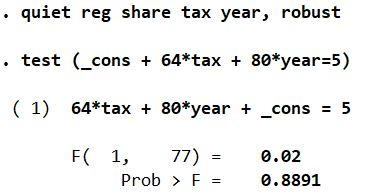
\includegraphics[width=0.45\textwidth]{heteFs.JPG}
    \end{figure}\\
    \item \textbf{Decision Rule}\\
    \begin{itemize}
        \item[$\square$] At $\alpha = 5\%$ and degrees of freedom $df_1 = q = 1$, $df_2 = n - k - 1 = 80 - 3 = 77$, the critical value $F_{1,77} = 3.9651$
        \item[$\square$] Heteroskedasticity-robust $F$-statistic $= 0.0196 < 3.9651$ and $p$-value $=0.8891 > 0.05$ $\Rightarrow$ We do not reject $H_0$ at 5\% significance level.
    \end{itemize}
    \item \textbf{Conclusion}\\
    Data do not contradict conjecture about income share in 2000 for a marginal tax rate of 64\%.
\end{itemize}
\end{frame}
%---------------------------------------------------------

%---------------------------------------------------------
\begin{frame}
\frametitle{Question (c)(cont.)}
\begin{itemize}
    \item \textbf{Test statistic} - \underline{Case 2.} Homokedasticity-only standard error:\\    
    \begin{figure}
        \centering
        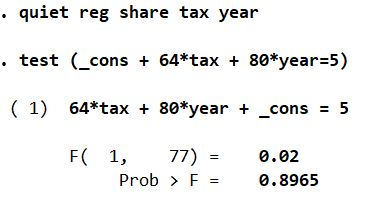
\includegraphics[width=0.45\textwidth]{homoFs.JPG}
    \end{figure}\\
    \item \textbf{Decision Rule}\\
    \begin{itemize}
        \item[$\square$] At $\alpha = 5\%$ and degrees of freedom $df_1 = q = 1$, $df_2 = n - k - 1 = 80 - 3 = 77$, the critical value $F_{1,77} = 3.9651$
        \item[$\square$] Homokedasticity-only $F$-statistic $= 0.0170 < 3.9651$ and $p$-value $=0.8965 > 0.05$ $\Rightarrow$ We still do not reject $H_0$ at 5\% significance level.
    \end{itemize}
    \item \textbf{Conclusion}\\
    Our conclusion does not change.
\end{itemize}
\end{frame}
%---------------------------------------------------------

%---------------------------------------------------------
\begin{frame}
\frametitle{Question (d)}
\begin{itemize}
    \item Test jointly the hypothesis in (c) and that a marginal tax rate of \textbf{64\%} in \textbf{1925} would have led to an expected income share of \textbf{5\%} for the top 1\% of income earners at 10\% level of significance.\\
\end{itemize}
\end{frame}
%---------------------------------------------------------

%---------------------------------------------------------
\begin{frame}
\frametitle{Question (d)(cont.)}
\begin{itemize}
    \item \textbf{Null hypothesis $H_0$:} 
    \begin{itemize}
        \item[$\square$] $H_0:$ A marginal tax rate of \textbf{64\%} would lead to the same \textbf{5\%} share for the top income earners in both \textbf{1925} and \textbf{2000}\\
        \vspace{2mm}
        $H_0: \beta_0 + 64 \beta_1 + 5 \beta_2 = 5 \; \text{ and } \; \beta_0 + 64 \beta_1 + 80 \beta_2 = 5$\\
        \vspace{2mm}
    \end{itemize}
    \vspace{3mm}
    \item \textbf{Alternative hypothesis $H_1$:}
    \begin{itemize}
        \item[$\square$] $H_1:$ at least one equality in $H_0$  does not hold\\
    \end{itemize}
\end{itemize}
\end{frame}
%---------------------------------------------------------

%---------------------------------------------------------
\begin{frame}
\frametitle{Question (d)(cont.)}
\begin{itemize}
    \item \textbf{Test statistic}   
    \begin{figure}
        \centering
        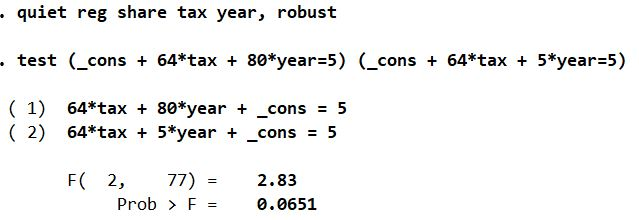
\includegraphics[width=0.65\textwidth]{joinFs.JPG}
    \end{figure}\\
    \item \textbf{Decision Rule}\\
    \begin{itemize}
        \item[$\square$] At $\alpha = 10\%$ and degrees of freedom $df_1 = q = 2$, $df_2 = n - k - 1 = 80 - 3 = 77$, the critical value $F_{2,77} = 2.3728$
        \item[$\square$] Heteroskedasticity-robust $F$-statistic $= 2.8314 > 2.3728$ and \\$p$-value $=0.0651 < 0.10$ $\Rightarrow$ We reject $H_0$ at 10\% significance level.
    \end{itemize}
    \item \textbf{Conclusion}\\
    We conclude that a marginal tax rate of 64\% does not lead to the same 5\% share for the top income earners in both 1925 and 2000.
\end{itemize}
\end{frame}
%---------------------------------------------------------


%---------------------------------------------------------
\begin{frame}
\frametitle{Question (e)}
\begin{itemize}
    \item Add the growth rate (\texttt{gwth}) to the equation in (b) and re-estimate. Interpret the estimated coefficient for \texttt{tax}.\\
%How is this coefficient affected by the inclusion of $gwth$?
%\item Using the equation estimated in part (e), estimate the year when $share$ will be smallest? Find a 95\% interval estimate for this year. Does the actual year with the smallest value for $share$ fall within the interval?
%\item Using the equation estimated in part (e), test the hypothesis that, in the year 2000, the expected income share of the top 1\% would have been 6\% if the marginal tax rate had been 64\% at that time .
%\item Using the equation estimated in part (e), test jointly the hypothesis in (f) and that a marginal tax rate of 64\% in 1925 would have led to an expected income share of 6\% for the top 1\% of income earners.
\pause
\vspace{3mm}
\textit{Answer.}
\begin{equation*}
    \underset{(se)}{\widehat{share}} = \underset{(0.2187)}{11.9728} - \underset{(0.01620)}{0.07548} \cdot tax - \underset{(0.01451)}{0.02928}\cdot year + \underset{(0.04199)}{0.08776}\cdot gwth
\end{equation*}\\
\end{itemize}
\end{frame}
%---------------------------------------------------------

%---------------------------------------------------------
\begin{frame}
\frametitle{Question (e)(cont.)}
\begin{itemize}
    \item Has adding the variable \texttt{gwth} led to substantial changes to your estimated coefficient for \texttt{tax}? \\
\pause
\vspace{3mm}
\textit{Answer.}

\begin{equation*}
    \underset{(se)}{\widehat{share}} = \underset{(0.2261)}{12.0370} - \underset{(0.01627)}{0.07467} \cdot tax - \underset{(0.01456)}{0.02776}\cdot year
\end{equation*}

\begin{equation*}
    \underset{(se)}{\widehat{share}} = \underset{(0.2187)}{11.9728} - \underset{(0.01620)}{0.07548} \cdot tax - \underset{(0.01451)}{0.02928}\cdot year + \underset{(0.04199)}{0.08776}\cdot gwth
\end{equation*}\\
\end{itemize}
\end{frame}
%---------------------------------------------------------

%---------------------------------------------------------
\begin{frame}
\frametitle{Question (e)(cont.)}
\begin{itemize}
    \item Can the changes, or lack of them, be explained by the correlations between \texttt{gwth} and the other variables in the equation?\\
    \item Why is \texttt{gwth} still included in the regression?\\
\pause
\vspace{3mm}
\textit{Answer.}
The lack of changes can be explained by the low correlations between \texttt{gwth} and the other regressors in the equation: 
$$\Corr(tax, gwth) =0.1849 \; \text{ and } \; \Corr(year, gwth)=0.1991$$
\end{itemize}
\end{frame}
%---------------------------------------------------------

%---------------------------------------------------------
\begin{frame}
\frametitle{Question (f)}
\begin{itemize}
    \item Test the overall significance of the following model at 1\% significance level:
$$share = \beta_0 + \beta_1tax + \beta_2year + \beta_3 gwth + e$$\\
    \pause
    \vspace{3mm}
    \textit{Answer.}\\
    To test the overall significance of the model:\\
    \vspace{3mm}
    $H_0: \beta_1 = 0 \; \text{and} \; \beta_2 = 0 \; \text{and}\; \beta_3 = 0$\\
    $\hspace{30mm}\text{vs. $H_1$ At least one of  }\beta_j \text{ is non-zero} \quad j=1,2,3$\\
    \vspace{3mm}
    Heteroskedasticity-robust $F$-statistic is 127.07 and $p$-value is 0.0000. At  $\alpha=0.01$, the critical value $F_{3,76}$ is 4.0503.\\
    \vspace{3mm}
    $\Rightarrow$ We reject $H_0$ at 1\% significance level and conclude at least one of the regressors has a statistically significant relationship with \texttt{share}. \end{itemize}
\end{frame}
%---------------------------------------------------------
%---------------------------------------------------------
\begin{frame}[fragile,t]
\linespread{1.3}
\frametitle{Testing of Joint Hypotheses}\label{Joint Hypotheses}

Procedure includes 5 steps:
\begin{itemize}
    \item Null hypothesis $H_0$
    \item Alternative hypothesis $H_1$
    \item Test statistic
    \item Decision rule
    \item Conclusion
\end{itemize}

\end{frame}
%---------------------------------------------------------

%---------------------------------------------------------
\begin{frame}[fragile,t]
\linespread{1.15}
\frametitle{Testing of Joint Hypotheses}
\begin{itemize}
    \item [$\blacksquare$] Null hypothesis $H_0$: imposes a restriction on two or more coefficients\\
    $$
    \text{e.g.} \quad H_0: \beta_1 = 0 \text{ and } \beta_2 = 0
    $$
    \item Alternative hypothesis $H_1$
    \item Test statistic
    \item Decision rule
    \item Conclusion
\end{itemize}

\end{frame}
%---------------------------------------------------------

%---------------------------------------------------------
\begin{frame}[fragile,t]
\linespread{1.15}
\frametitle{Testing of Joint Hypotheses}


Procedure includes 5 steps:
\begin{itemize}
    \item [$\blacksquare$] Null hypothesis $H_0$: imposes a restriction on two or more coefficients\\
    $$
    \text{e.g.} \quad H_0: \beta_1 = 0 \text{ and } \beta_2 = 0
    $$
    \item [$\blacksquare$] Alternative hypothesis $H_1$:
    $$
    \text{e.g.} \quad H_0: \beta_1 \neq 0 \text{ or } \beta_2 \neq 0 \text{ or both are non-zero}
    $$ 
    \item Test statistic
    \item Decision rule
    \item Conclusion
\end{itemize}

\end{frame}
%---------------------------------------------------------
%---------------------------------------------------------
\begin{frame}[fragile,t]
\linespread{1.15}
\frametitle{Testing of Joint Hypotheses}
\begin{itemize}
    \item Null hypothesis $H_0$
    \item Alternative hypothesis $H_1$
    \item [$\blacksquare$] Test statistic:
    $$
    \textbf{\text{F-statistic}} =\frac{\left(S S R_{R}-S S R_{U}\right) / q}{S S R_{U} /(n-k-1)}  =\frac{\left(R_{U}^{2}-R_{R}^{2}\right) / q}{\left(1-R_{U}^{2}\right) /(n-k-1)}
    $$
    Where: 
    \begin{itemize}
        \item [$\square$] \textcolor{red}{n}: number of observations
        \item [$\square$] \textcolor{red}{k}: number of regressors (independent variables) under the unrestricted model
        \item [$\square$] \textcolor{red}{k+1}: number of parameters under the unrestricted model (= number of estimated coefficients)
        \item [$\square$] \textcolor{red}{q}: number of restrictions (number of linear hypotheses with \textbf{equal} sign)
    \end{itemize}
    \item Decision rule
    \item Conclusion
\end{itemize}

\end{frame}
%---------------------------------------------------------

%---------------------------------------------------------
\begin{frame}[fragile,t]
\linespread{1.15}
\frametitle{Testing of Joint Hypotheses}
\begin{itemize}
    \item Null hypothesis $H_0$
    \item Alternative hypothesis $H_1$
    \item [$\blacksquare$] Test statistic:
    $$
    \textbf{\text{F-statistic}} =\frac{\left(S S R_{R}-S S R_{U}\right) / q}{S S R_{U} /(n-k-1)}  =\frac{\left(R_{U}^{2}-R_{R}^{2}\right) / q}{\left(1-R_{U}^{2}\right) /(n-k-1)}
    $$
    Follows a $F_{q,n-k-1}$ distribution with degrees of freedom $df_1 = q$ and $df_2 = n - k - 1$. 
    \item Decision rule
    \item Conclusion
\end{itemize}

\end{frame}
%---------------------------------------------------------

%---------------------------------------------------------
\begin{frame}[fragile,t]
\linespread{1.15}
\frametitle{F-distribution}
\begin{figure}
    \centering
    \includeg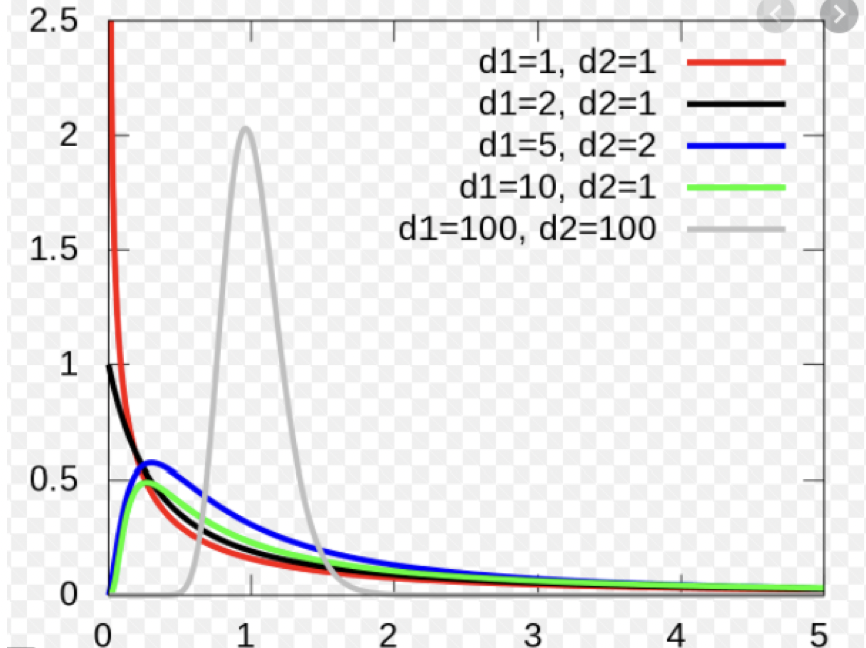
\includegraphics[scale = 0.5]{Fstats.png}
    \caption{}
    \label{fig:my_label}
\end{figure}
\end{frame}
%---------------------------------------------------------

%---------------------------------------------------------
\begin{frame}[fragile,t]
\linespread{1.15}
\frametitle{Testing of Joint Hypotheses}
\begin{itemize}
    \item Null hypothesis $H_0$
    \item Alternative hypothesis $H_1$
    \item Test statistic
    \item [$\blacksquare$] Decision rule:
    \begin{itemize}
        \item [$\square$] What is the \textbf{significance level} $\alpha$?\\
        $\Longrightarrow$ Usually chosen to be 0.01, 0.05 or 0.10.
        \item [$\square$] Is the decision rule based on \textcolor{green}{\textbf{critical values}} or \textcolor{red}{\textbf{p-value}}?\\
        $\Longrightarrow$ Distinguish...
    \end{itemize}
    \item Conclusion
\end{itemize}

\end{frame}
%---------------------------------------------------------

%---------------------------------------------------------
\begin{frame}[fragile,t]
\frametitle{Decision Rule}
\begin{itemize}
    \item [$\square$] Approach 1: \textcolor{green}{\textbf{Critical-value Test}}\\
\quad Reject $H_0$ if $\text{F-statistic } > \text{ Critical value } F_\alpha$\\
   \item [$\square$] Approach 2: \textcolor{red}{\textbf{p-value Test}}\\
\quad Reject $H_0$ if $\text{p-value }\leq \alpha$
\end{itemize}
\begin{figure}
    \centering
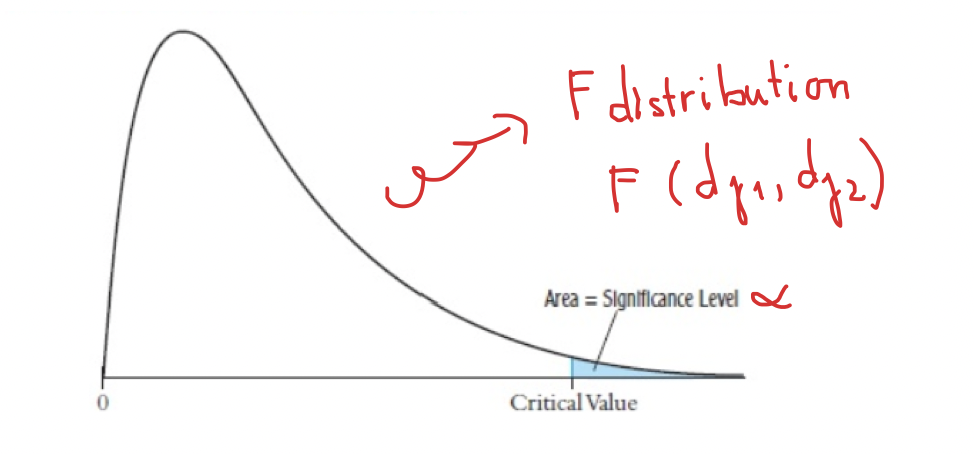
\includegraphics[scale = 0.4]{DecisionRule.png}\\
    \caption{}
\end{figure}
\end{frame}
%---------------------------------------------------------

%---------------------------------------------------------
\begin{frame}[fragile,t]
\linespread{1.3}
\frametitle{Testing of Joint Hypotheses}

Procedure includes 5 steps:
\begin{itemize}
    \item Null hypothesis $H_0$
    \item Alternative hypothesis $H_1$
    \item Test statistic
    \item Decision rule
    \item [$\blacksquare$] Conclusion:
    \begin{itemize}
        \item [$\square$] Do you \textit{reject} or or \textit{fail to reject} the null hypothesis at the significance level $\alpha$?
        \item [$\square$] AVOID saying that you "\textit{accept}" the null hypothesis, which can be very misleading
    \end{itemize}
\end{itemize}
\hyperlink{Back}{\beamerbutton{Back}}
\end{frame}
%---------------------------------------------------------
\end{document}